\chapter{Optimised Loading of Change-based Model Persistence}
\label{ch:optimised_loading}

This chapter introduces and evaluates an efficient approach for loading models stored in a change-based format. The work builds on the change-based model persistence format presented in Chapter 3. It also presents the evaluation on the performance of the proposed loading approach and the assessment of its impact on saving change-based models. The results show that the proposed approach significantly improves loading times compared to the baseline change-based persistence loading approach, and has a negligible impact on saving.

\section{Introduction}
\label{sec:introduction_4}
Saving a model in change-based persistence typically results in a large, ever-growing file (see Table \ref{table:advantages_drawbacks}) since every change made to the model (even model element deletions) is appended to the file. This is also applies to the implementation of change-based model persistence (CBP) in this work that uses a text file to simplify saving changes by appending them and reading them into memory. The increasing records of changes also causes its loading time to increase, as the loading process has to reconstruct the model's current state from its history \cite{DBLP:conf/models/YohannisKP17}. This chapter proposes and evaluates an approach that reduces CBP model loading time by avoiding the replaying of historical changes that have no impact on the final state of the model.

The rest of this chapter is structured as follows. Section \ref{sec:case_study} introduces a running example.
Section \ref{sec:loading_time_optimisation} presents the approach to speed up model loading and its supporting data structures. Section \ref{sec:evaluation_4} presents experimental results and evaluation.  Section \ref{sec:conclusions_4} concludes this chapter.

\section{Running Example}
\label{sec:case_study}
To explain the optimised loading algorithm for change-based models proposed in this chapter, instead of using the running example introduced in Section \ref{sec:running_example_1}, a minimal tree metamodel and example tree models in Figure \ref{fig:tree_example} are used to simplify explaining the approach.
 
The metamodel for the minimal tree model is expressed in the Eclipse Modelling Framework (EMF) Ecore metamodelling language, the de-facto standard for object-oriented metamodelling.  The example is contrived to avoid unnecessary repetition, whilst providing adequate coverage of the core features of Ecore (classes, single/multi-valued features, references).
In this example, a tree model consists of named nodes which can -- optionally -- contain other nodes (\textsf{child} reference). 

\begin{figure}[ht]
\begin{subfigure}[t]{0.32\linewidth}
\centering
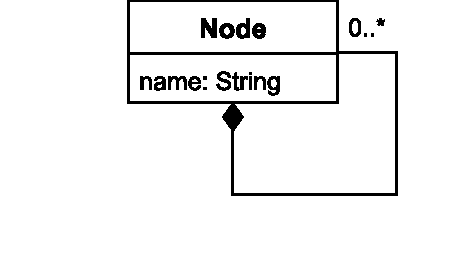
\includegraphics[width=\linewidth]{node_metamodel}
\caption{the tree metamodel (EMF/Ecore)}
\label{fig:tree_metamodel}
\end{subfigure}
\hfill
\begin{subfigure}[t]{0.32\linewidth}
\centering
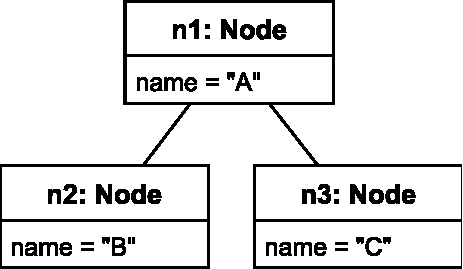
\includegraphics[width=\linewidth]{initial_chart_1}
\caption{the initial state of a tree model}
\label{fig:initial_model}
\end{subfigure}
\hfill
\begin{subfigure}[t]{0.32\linewidth}
  \centering
  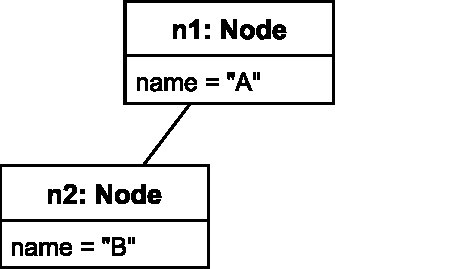
\includegraphics[width=\linewidth]{initial_chart_2}
  \caption{the eventual state after \textsf{n3} is deleted}
  \label{fig:modified_model}
\end{subfigure}
\caption{Running example of a metamodel and a conformant model.}
\label{fig:tree_example}
\end{figure}

The initial state of the model in Figure \ref{fig:initial_model} has three nodes, \textsf{n1}, \textsf{n2}, and \textsf{n3}. It was initially constructed by firstly creating the three nodes (\textsf{n1}, \textsf{n2}, and \textsf{n3}) and nodes \textsf{n2} and \textsf{n3} were added as children of \textsf{n1}. The model then was modified by deleting node \textsf{n3} producing the eventual state in Figure \ref{fig:modified_model}.

\vspace{-20pt}
\begin{minipage}[t]{0.49\linewidth}
\begin{lstlisting}[style=xmi,caption={State-based representation in simplified XMI of the tree model in Figure \ref{fig:initial_model}.},label=lst:xmimodel_0]
<Node id="n1" name="A">
  <children id="n2" name="B"/>
  <children id="n3" name="C"/>
</Node>
\end{lstlisting}
\end{minipage}
\hfill
\begin{minipage}[t]{0.49\linewidth}
\begin{lstlisting}[style=xmi,caption={State-based representation in simplified XMI of the tree model in Figure \ref{fig:modified_model}.},label=lst:xmimodel]
<Node id="n1" name="A">
  <children id="n2" name="B"/>
</Node>
\end{lstlisting}
\end{minipage}

\vspace{-20pt}
\begin{minipage}[t]{0.49\linewidth}
\begin{lstlisting}[style=eol,caption={Change-based representation of the tree model in Figure \ref{fig:initial_model}.},label=lst:cbpmodel_0]
create n1 of Node
set n1.name from null to "A"  
create n2 of Node
set n2.name from null to "B"  
create n3 of Node
set n3.name from null to "C"  
add n2 to n1.children at 0  
add n3 to n1.children at 1
\end{lstlisting}
\end{minipage}
\hfill
\begin{minipage}[t]{0.49\linewidth}
  \begin{lstlisting}[style=eol,caption={Change-based representation of the tree model in Figure \ref{fig:modified_model}.},label=lst:cbpmodel]
create n1 of Node
set n1.name from null to "A"  
create n2 of Node
set n2.name from null to "B"  
create n3 of Node
set n3.name from null to "C"  
add n2 to n1.children at 0  
add n3 to n1.children at 1
remove n3 from n1.children at 1
delete n3
\end{lstlisting}
\end{minipage}

Listings \ref{lst:xmimodel_0} and \ref{lst:xmimodel} show the simplified XMI format of the models in Figures \ref{fig:initial_model} and \ref{fig:modified_model} when they are persisted in state-based representation. Listings \ref{lst:cbpmodel_0} and \ref{lst:cbpmodel} show the change-based representation of both models respectively, using the CBP syntax introduced in Chapter \ref{ch:change_based_model_persistence}. As can be seen in both change-based representation, lines 1-6 record the creation and naming of the three nodes, and lines 7-8 record the addition of \textsf{n2} and \textsf{n3} as children of \textsf{n1}. Change-based representation in Listing \ref{lst:cbpmodel} records two additional rows since it also records the recent changes that produce the eventual state of the tree model in Figure \ref{fig:modified_model}. Lines 9-10 capture the deletion of \textsf{n3} (the \textsf{remove} command removes f \textsf{n3} from its container, and the $delete$ command completely removes \textsf{n3} from its model). Changes in a CBP representation can be uniquely identified by their line numbers.

The example model history illustrates a case where  earlier events (creating \textsf{n3} in line 5, naming it in line 6, making it a child of \textsf{n1} in line 8, removing it from the container in line 9) are superseded by a subsequent event (deletion of \textsf{n3} in line 10).  Loading of the eventual model would arguably be faster if the events in lines 5, 6, 8, 9 and 10 could be ignored.

%\vspace{-10pt}
\section{Towards Efficient Loading of Change-Based Models}
\label{sec:loading_time_optimisation}

%\vspace{-10pt}
The flowchart in Figure \ref{fig:flowchart} provides an overview of the editing lifecycle of a CBP model \cite{DBLP:conf/models/YohannisKP17}, with the proposed extensions shown as starred blocks. A model is loaded (1), edited (2) and saved (3).  During editing, the changes made to the model are recorded in a memory-based data structure, serialised and with the latest events appended at the end (4). The change events are persisted into a CBP file every time the model is saved (5). When a model is re-loaded, the current model state is recreated by replaying the events stored in the CBP file (6).

\begin{figure}[ht]
\centering
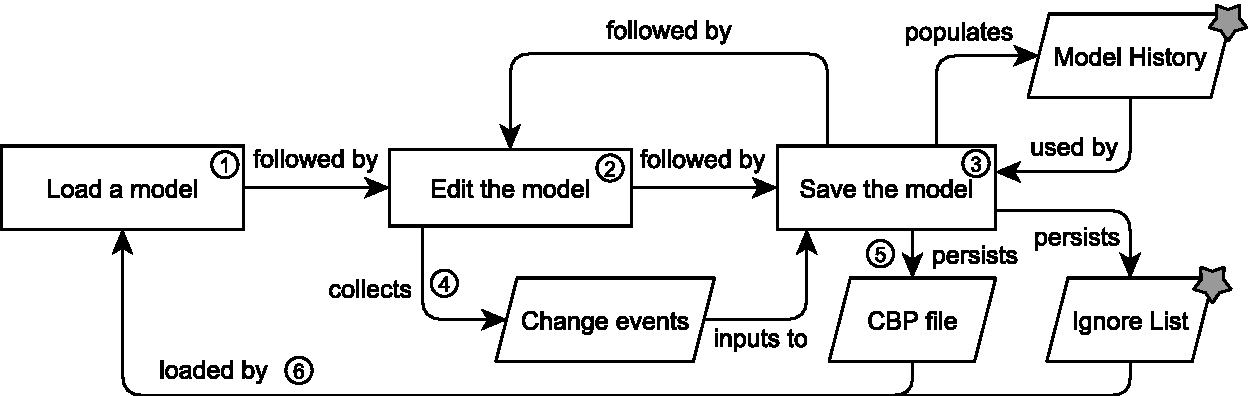
\includegraphics[width=\linewidth]{flowchart}
\caption{CBP workflow, with optimised loading elements indicated by starred blocks.}
\label{fig:flowchart}
\end{figure}

As mentioned in Section \ref{sec:proposed_approach}, the editing history recorded in a CBP file is immutable. As such, superseded events cannot be simply removed from the CBP file. Therefore, the proposed approach adds two artefacts: an in-memory \textit{Model History} data structure which aggregates change events per model element, and an \textit{Ignore List} file, which persists the position (i.e. line numbers) of superseded events so that the events can be ignored the next time the model is loaded. The Ignore List is saved alongside the CBP file. The rest of this section presents how the Model History is used to detect superseded events and generate the Ignore List.

\subsection{Model History}
\label{subsec:model_history}
The Model History data structure stores events and their line numbers in a CBP representation.  The data can be used to reason about the events of a particular element and to determine which events are superseded. The line number in the CBP representation is referred as the \textit{event number}. The proposed data structure is defined in Figure \ref{fig:object_history} using a class diagram.  

A \textsf{ModelHistory} has a \textsf{URI} attribute to identify the model for which it records changes.  A \textsf{ModelHistory} can link to many \textsf{ElementHistory} objects, each identified by its \textsf{element} field which is queried from the model. An \textsf{ElementHistory} can link to many \textsf{FeatureHistories}, representing the editing histories of individual features -- either references or attributes of the element. A \textsf{FeatureHistory} has a \textsf{type} (attribute or reference) and a \textsf{name}, identifying the feature.

%\vspace{-20pt}    
\begin{figure}[ht]
\centering
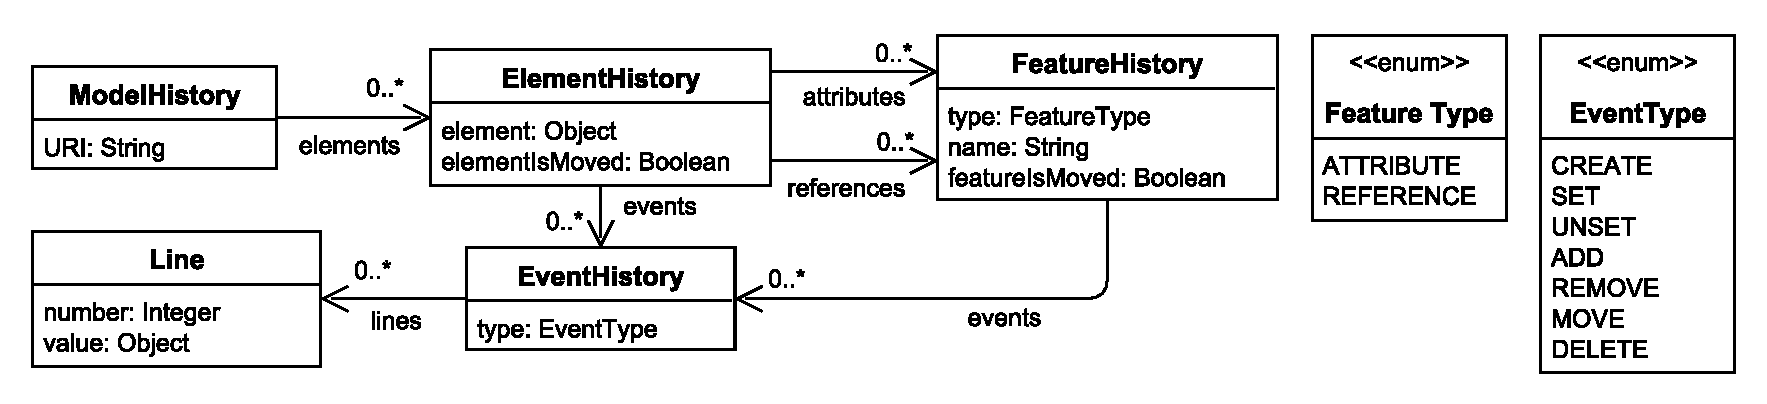
\includegraphics[width=\linewidth]{object_history}
\caption{The class model defining Model History.}
\label{fig:object_history}
\end{figure}

%\vspace{-30pt}
\begin{figure}[ht]
\centering
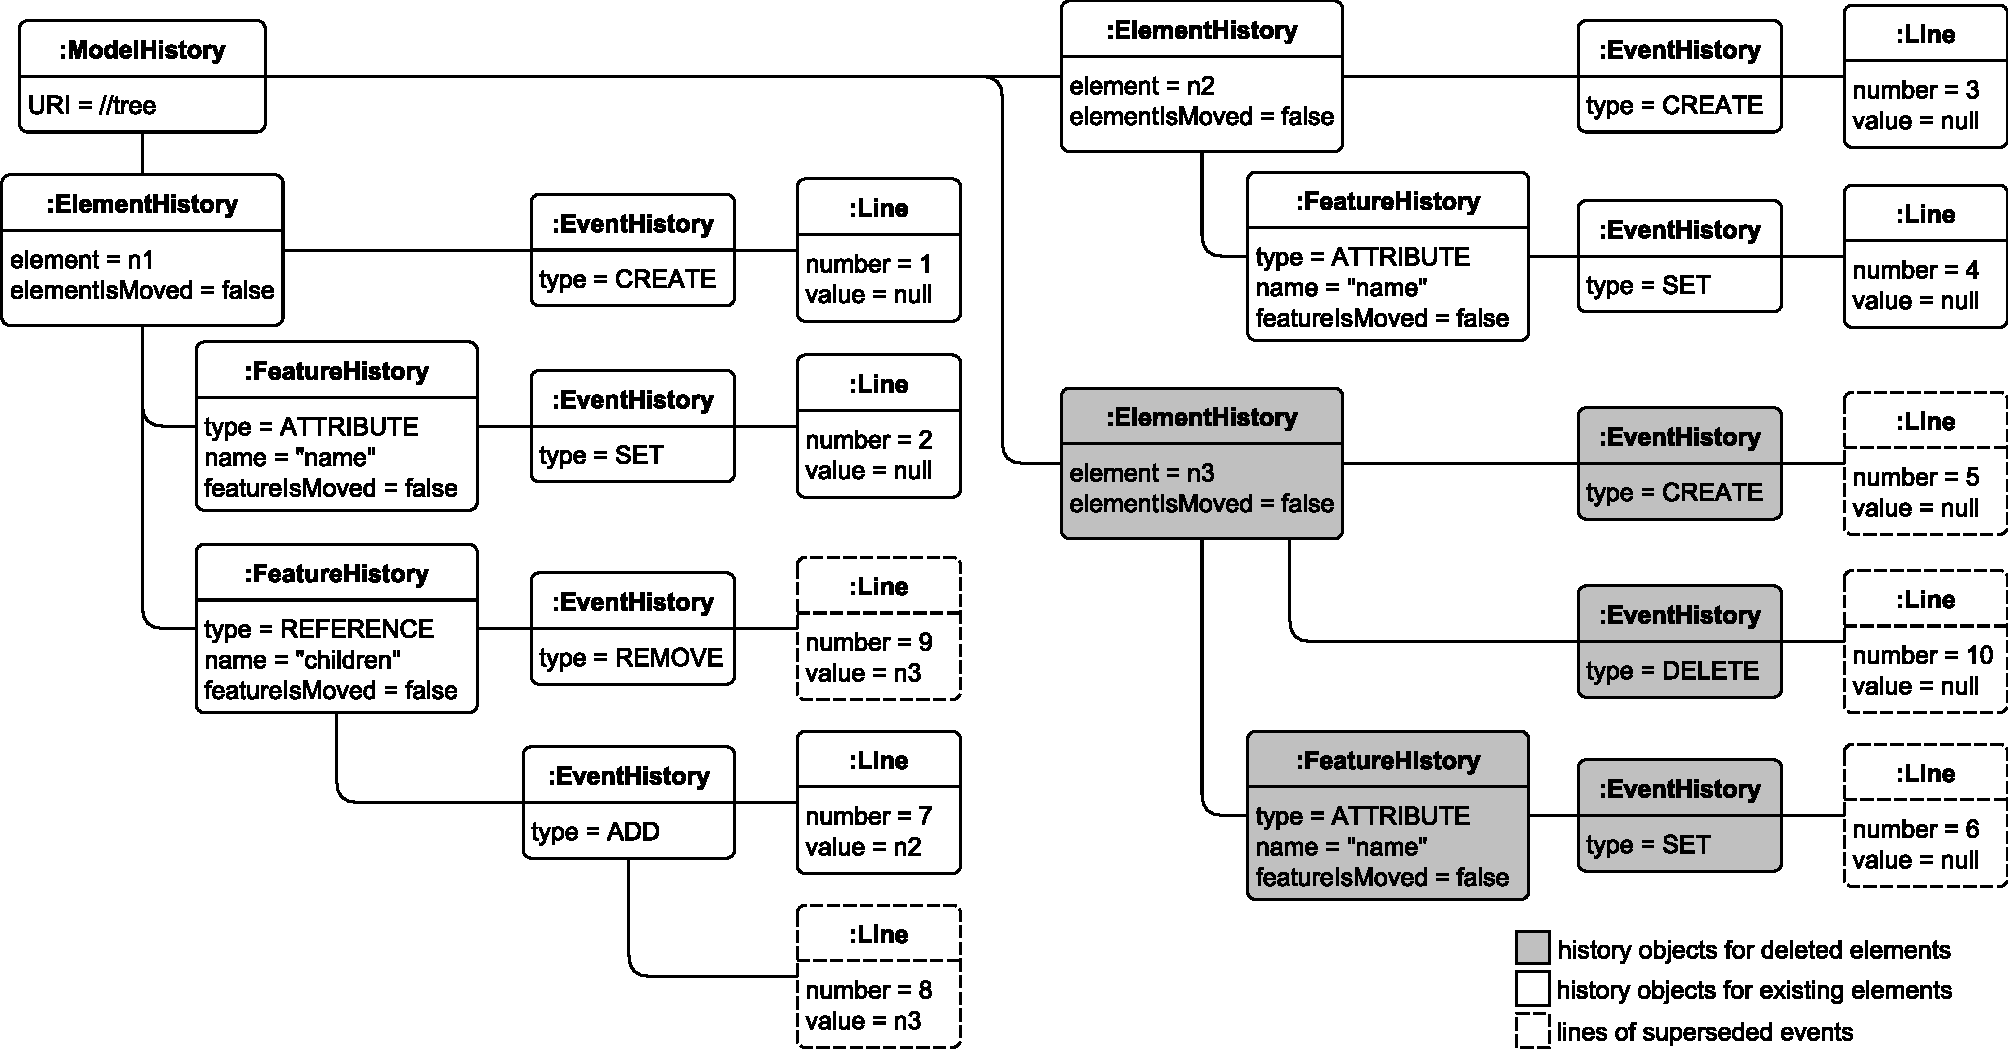
\includegraphics[width=\linewidth]{history_structure}
\caption{The object diagram of the CBP model history in Listing \ref{lst:cbpmodel}.}
\label{fig:history_structure}
\end{figure}

An \textsf{EventHistory} represents series of events of the same type; it has an attribute \textsf{type} to identify the events' type and can have many \textsf{Line}s. A \textsf{Line} has a \textsf{number} attribute, to record the event number and a \textsf{value} that records the element involved in the event (Value is only used for events with types \textsf{add}, \textsf{remove} and \textsf{move}). Each \textsf{FeatureHistory} can have many \textsf{EventHistories}, to represent the events that modify the values of the features. Each \textsf{ElementHistory} can have many \textsf{EventHistories} to represent events that affect the state of the elements (life-cycle and relations to multivalued features). Figure \ref{fig:history_structure} shows an object diagram corresponding to the model in Figure \ref{fig:object_history} that captures the model history shown in Listing \ref{lst:cbpmodel}. The grey rectangles are \textsf{History} objects related to the deleted node \textsf{n3}. The rectangles with the dashed outline are \textsf{Line} objects that represent superseded changes. 

The following section presents the different strategies used to identify superseded events that will be added to the Ignore List.   

%\vspace{-10pt}
\subsection{Set and Unset Events}
\label{subsec:set_and_unset_operations}
During the lifecycle of a model, a single-valued feature can have its value set (assigned) or unset many times. Each event is persisted, but only the last assigned value needs to be considered. For example, in Listing \ref{lst:set_unset_example_1}, the feature \textsf{name} is set to the value ``A'', unset, and finally set to the value ``B''.  In the final state of the model, \textsf{n1.name} = ``B''. Thus, only line 4 is significant for the model's final state and therefore lines 2 and 3 can be ignored when loading the model. For a \textsf{set} event, all preceding \textsf{set} and \textsf{unset} events can be ignored, but for an \textsf{unset} event, all \textsf{set} and \textsf{unset} events can be ignored. Executing it does not have any effect on the final state of a model if all the preceding events also have been ignored.

\vspace{-20pt}
\begin{minipage}[t]{0.49\linewidth}
\begin{lstlisting}[style=eol,caption={A CBP representation of attribute \textsf{name} assignments ended with SET.},label=lst:set_unset_example_1]
create n1 of Node
set n1.name from null to "A"
unset n1.name from "A" to null
set n1.name from null to "B"
\end{lstlisting}
\end{minipage}
\hfill
\begin{minipage}[t]{0.49\linewidth}
\begin{lstlisting}[style=eol,caption={A CBP representation of attribute \textsf{name} assignments ended with UNSET.},label=lst:set_unset_example_2]
create n1 of Node
set n1.name from null to "A"
set n1.name from null to "B"
unset n1.name from "B" to null
\end{lstlisting}
\end{minipage}

Based on the Listing \ref{lst:set_unset_example_1}, our approach creates an instance of \textsf{ElementHistory} \textsf{n1} which contains an instance of \textsf{FeatureHistory} \textsf{name}. The \textsf{FeatureHistory} \textsf{name} consists of two \textsf{EventHistory} instances, with types \textsf{set} and \textsf{unset} (the instances are named \textsf{set} and \textsf{unset} respectively for brevity). The \textsf{set} records the $Line$ instances that hold the event numbers of the \textsf{set} events, and similarly for \textsf{unset}.

From Listing \ref{lst:set_unset_example_1}, we can thus infer that \textsf{name}.\textsf{set}.\textsf{lines} = $\{2,4\}$ and \textsf{name}.\textsf{unset}. \textsf{lines} = $\{3\}$. The event numbers in both lists are used to determine that the events represented by lines 2 and 3 are superseded by that in line 4, which is a \textsf{set} event, giving an \textsf{ignoreList} = $\{2, 3\}$.  By the same process, for Listing \ref{lst:set_unset_example_2}, we can reason that \textsf{name}.\textsf{set}.\textsf{lines} = \{2,3\} and \textsf{name}.\textsf{unset}.\textsf{lines} = \{4\}.  However, this case, the highest-numbered event is an \textsf{unset}, all so line numbers are put into the ignoreList (\textsf{ignoreList} = $\{2, 3, 4\}$) (\textsf{unset} event can be ignored along with all preceding {\textsf{set} and \textsf{unset} events). 

%\vspace{-10pt}
\subsection{Add, Remove, and Move Events}\label{subsec:add_remove_and_move_operations}
For a multi-valued feature, add, remove, and move events can be called many times, to modify the feature. If an element is added to the feature, moved multiple times, and finally removed, then all the element's preceding events can be ignored, as long as the order of the feature's elements is not changed. 

Listing \ref{lst:add_move_reference} shows an example without a \textsf{move} event. In this example, nodes \textsf{n1}, \textsf{n2}, and \textsf{n3} are added to the \textsf{children} feature of \textsf{p} (lines 5-7). In the latest state of the model, \textsf{children} only contains \textsf{n1} and \textsf{n3}. As a result, the loading process could ignore the events that represent the \textsf{add} and \textsf{remove} events on \textsf{n1}. 

\vspace{-20pt}
\begin{lstlisting}[style=eol,caption={A CBP of add and remove operations.},label=lst:add_move_reference]
create p of Node                // children = []
create n1 of Node               // children = []
create n2 of Node               // children = []
create n3 of Node               // children = []
add n1 to p.children at 0       // children = [n1]
add n2 to p.children at 1       // children = [n1, n2]
add n3 to p.children at 2       // children = [n1, n2, n3]
remove n2 from p.children at 1  // children = [n1, n3]   
\end{lstlisting}

\begin{lstlisting}[style=eol,caption={A CBP representation of add, move, and remove operations.},label=lst:add_remove_move_reference]
create p of Node                    // children = []          
create n1 of Node                   // children = []         
create n2 of Node                   // children = []         
create n3 of Node                   // children = []
add n1 to p.children at 0           // children = [n1]
add n2 to p.children at 1           // children = [n1, n2]
add n3 to p.children at 2           // children = [n1, n2, n3]
move n1 in p.children from 0 to 1   // children = [n2, n1, n3] 
remove n2 from p.children at 0      // children = [n1, n3]
\end{lstlisting}

To create the Ignore List for Listing \ref{lst:add_move_reference}, we can deduce that \textsf{children}.\textsf{add}.\textsf{lines} = \{\{5, \textsf{n1}\}, \{6, \textsf{n2}\} \{7, \textsf{n3}\}\} (5 is the line number and \textsf{n1} is the value) and \textsf{children}.\textsf{remove}.\textsf{lines} = \{\{8, \textsf{n1}\}\}. Since \textsf{n2} is removed from its containing feature (line 8), then executing its preceding add and remove events is unnecessary. Note that we retain the \textsf{create} event (line 3) as \textsf{n2} has not been deleted from the model -- only removed from its containing feature. We can iterate through the add and move structures to identify the events on \textsf{n2} that should be removed, resulting in the \textsf{ignoreList} = \{6, 8\}.

Listing \ref{lst:add_remove_move_reference} shows an example with a \textsf{move} event\footnote{The commented parts  show the end states of \textsf{children} after each event}. Let's say that a \textsf{move} event is inserted at line 8 (this insertion shifts the \textsf{remove} event of \textsf{n2} from line 8 to line 9). With the introduction of this \textsf{move} event, we now have the \textsf{children}.\textsf{add}.\textsf{lines} = \{\{5, \textsf{n1}\}, \{6, \textsf{n2}\} \{7, \textsf{n3}\}\}, \textsf{children}.\textsf{move}.\textsf{lines} = \{\{8, \textsf{n1}\}\}, and \textsf{children}.\textsf{remove}.\textsf{lines} = \{\{9, \textsf{n2}\}\}. In the final state of the model, \textsf{children} should have \textsf{n1} and \textsf{n3} in order, \textsf{children} = [n1, n3].  

However, executing the previous strategy naively leads to an erroneous final state. Using \textsf{ignoreList} = \{6, 8\} produced by the naive strategy leads to a different order of \textsf{n1} and \textsf{n3} in the final state of the model where \textsf{children} = [n3, n1] as shown by the naive optimised CBP in Listing \ref{lst:naive_add_remove_move_reference}. To overcome this problem, *$IsMoved$ flags in Figure \ref{fig:object_history} is used to sign  features and elements if they have been moved -- the flags are set to $true$. If an element's *$IsMoved$ flag is true then all of its line numbers related to \textsf{add}, \textsf{move}, \textsf{remove} events cannot be put into the \textsf{ignoreList}. The flags are set to $false$ if the feature is empty. 

\vspace{-20pt}
\begin{lstlisting}[style=eol,caption={A naive optimised CBP representation of original CBP representation in Listing \ref{lst:add_remove_move_reference} .},label=lst:naive_add_remove_move_reference]
create p of Node                    // children = []
create n1 of Node                   // children = []
create n2 of Node                   // children = []
create n3 of Node                   // children = []
add n1 to p.children at 0           // children = [n1]
add n3 to p.children at 1           // children = [n1, n3]
move n1 in p.children from 0 to 1   // children = [n3, n1]
\end{lstlisting}

\subsection{Create and Delete Events}
\label{subsec:create_and_delete_operations}

When an element is deleted, it is completely removed from the model. Therefore, all previous events ($create$, \textsf{set}, \textsf{unset}, \textsf{move}, \textsf{add}, \textsf{remove}, $delete$) on features of the element can be ignored. For example, when node \textsf{n3} in Listing \ref{lst:cbpmodel} is deleted, the events in lines 5-6 and 8-10 are superseded. If the Listing \ref{lst:cbpmodel} is optimised -- some of its events are ignored -- when loading, it runs as if the Listing \ref{lst:cbpmodel_optimised} are executed.

\vspace{-20pt}
\begin{lstlisting}[style=eol,caption={Change-based representation of the model in Figure \ref{fig:tree_example} after removal of node \textsf{n3}.},label=lst:cbpmodel_optimised]
create n1 of Node
set n1.name from null to "A"
create n2 of Node
set n2.name from null to "B"
add n2 to n1.children at index 0
\end{lstlisting}

Using the Listing \ref{lst:cbpmodel}, we can construct the structure of histories that are related to element \textsf{n3} as follows: \textsf{n3}.$create$.\textsf{lines} = \{5\}, \textsf{n3}.\textsf{name}.\textsf{set}.\textsf{lines} = \{6\}, \textsf{n1}.\textsf{children}.\textsf{add}.\textsf{lines} = \{\{7, \textsf{n2}\}, \{8, \textsf{n3}\}\}, \textsf{n1}.\textsf{children}.\textsf{remove}.\textsf{lines} = \{\{9, \textsf{n3}\}\}, and \textsf{n3}.$delete$.\textsf{lines} = \{10\}. Thus, when element \textsf{n3} is deleted, by iterating through all these history structures, all line numbers associated with \textsf{n3} can be identified and added to \textsf{ignoreList} producing \textsf{ignoreList} = \{5 6, 8, 9, 10\} so they can be ignored in the next model loading.

\section{Evaluation}
\label{sec:evaluation_4}

This work has developed the proposed efficient loading approach on top of the original CBP implementation \cite{DBLP:conf/models/YohannisKP17,epsilonlabs2019emfcbp} and evaluated our approach's model loading performance, as well as its memory footprint and its impact on the time required to save changes made to CBP models. The evaluation was performed on Intel\textsuperscript{\textregistered} Core\textsuperscript{TM} i7-6500U CPU@2.50GHz 2.59GHz, 12GB RAM, and the Java\textsuperscript{TM} SE Runtime Environment (build 1.8.0\textunderscore162-b12).

Given that CBP is a very recent contribution and we are not aware of any existing datasets containing real-world models expressed in a change-based format, this work has used synthetic change-based models for the experiments. The synthetic models were derived from real-world data sources: the BPMN2 \cite{eclipse2017bpmn2,eclipse2018bpmn2git} and Epsilon \cite{eclipse2017epsilon,eclipse2018epsilongit} software projects, and the United States article \cite{wikipedia2018us} on Wikipedia (the article is further referred as Wikipedia). For the first two projects, for each version of the cases, MoDisco \cite{DBLP:journals/infsof/BruneliereCDM14} was used to generate a UML2 \cite{eclipse2017uml2} model that reflects its source code. For the Wikipedia article, a model that conforms to the Modisco XML metamodel \cite{eclipse2018modiscoxml} was generated. Since these cases have many versions -- represented by commits/revisions, different models of the versions can be generated, and to some degree, they reflect the time-ordered changes of the cases. The synthetic change-based model for each case was derived by comparing an initially-empty running model to different versions of the case's models sequentially. All identified differences were then reconciled by performing a unidirectional merging to the running model. All changes made to the running model during the merging process were captured and persisted into a CBP file. EMF Compare was used \cite{eclipse2017compare} to perform the comparison and merging.

Using the synthetic models, evaluation was conducted on loading time, saving time, and memory footprint for both loading and saving. To compare the loading time, we ran the optimised and original (baseline) CBP algorithms to reconstruct the current state of each of the three models (the results are shown in Figure \ref{fig:loadtime}). As discussed in Section \ref{sec:loading_time_optimisation}, optimised CBP also does extra work when saving the changes to a model, in order to save time (relative to original CBP) when loading a model. To analyse the performance effect of optimisation activities, we, therefore, compared the overall time required to save a new version of the models described above, after one single change has been made (The results are shown in Figure \ref{fig:savetime}). This work also compared the memory footprints for both loading and saving since the optimised CBP approach also requires the maintenance of an additional in-memory data structure that keeps track of element and feature editing histories (see Figure \ref{fig:loadmemory} and \ref{fig:savememory} for the results). 

For each combination of dimensions (loading time, saving time, loading memory footprint, saving memory footprint),  persistence types (original CBP, optimised CBP, and XMI), and cases (BPMN2, Epsilon, and Wikipedia), we performed measurement 22 times. The results of the measurement enabled us to perform the Welch's t-test \cite{welch1947ttest} to find the significance of the comparisons for each case. This evaluation used a significance level of 5\%. If t-test' $p$-$value$ $<$ 0.05, the null hypothesis -- the $means$ of the compared persistence types are equal ($H_0$) -- is rejected and the alternative hypothesis -- the $means$ of the compared persistence types are not equal ($H_1$) -- is accepted.

For loading and saving time, this work measured the delta time required to complete the loading and saving. For memory footprint, this work measured the delta of memory used before and after loading and saving completes. The results are presented below.

\subsection{Data Description}
\label{subsec:data_description}

\begin{table} [ht]
\centering
\caption{Description of change-based models generated for evaluation.}
\label{table:data_description}
\begin{tabular}{>{\centering\arraybackslash}p{1.5cm}>{\centering\arraybackslash}p{1.7cm}>{\centering\arraybackslash}p{1.7cm}>{\centering\arraybackslash}p{1.6cm}
>{\centering\arraybackslash}p{1.5cm}>{\centering\arraybackslash}p{2cm}}
\hline 
\textbf{Model} & \textbf{Total Events} & \textbf{Ignored Events} & \textbf{Elements} & \textbf{Total Versions} & \textbf{Processed Versions} \\
\hline
BPMN2 & \multicolumn{1}{r}{1.2 million} & \multicolumn{1}{r}{1.1 million} & \multicolumn{1}{r}{62,062} & \multicolumn{1}{r}{192} & \multicolumn{1}{r}{192 (100.0\%)} \\
Epsilon & \multicolumn{1}{r}{2.6 million} & \multicolumn{1}{r}{1.8 million} & \multicolumn{1}{r}{79,459} & \multicolumn{1}{r}{3,037} & \multicolumn{1}{r}{727 (23.9\%)} \\
Wikipedia & \multicolumn{1}{r}{11.5 million} & \multicolumn{1}{r}{7.8 million} & \multicolumn{1}{r}{12,144} & \multicolumn{1}{r}{37,996} & \multicolumn{1}{r}{3,100 (8.2\%)} \\
\hline 
\end{tabular}
\end{table}

Table \ref{table:data_description} summarises events, elements and saved versions for the Epsilon, BPMN2, and Wikipedia cases. $Total$ $Events$ is the numbers of events that were produced by our approach in generating a change-based model for each case.  $Ignored$ $Events$ is the number of superseded events that do not need to be replayed when reloading the models. $Elements$ is the number of elements contained in each model. $Total$ $Versions$ is the number of commits/revisions made to the cases, taken from the git repositories or Wikipedia at the time this evaluation performed. $Processed$ $Versions$ is the number of commits/revisions that were processed to produce change-based models: since the comparison between versions takes considerable time, not all versions are processed here.

\subsection{Model Loading Time}
\label{subsec:loading_time_test}
This section presents the results of the loading time measurement of change-based models for each pair of the persistence types and cases, and the t-test results of their comparisons (Table \ref{table:ttest_results_loadtime} and Figure \ref{fig:loadtime}). 

\begin{table}[ht]
\footnotesize
\centering
\caption{The t-test results of loading time comparison between original CBP (CBP), optimised CBP (OCBP), and XMI.}
\label{table:ttest_results_loadtime}
\begin{tabular}
{|p{0.08\textwidth}p{0.08\textwidth}p{0.09\textwidth}|p{0.18\textwidth}p{0.10\textwidth}p{0.06\textwidth}p{0.08\textwidth}|}
\hline 
% BPMN2 Load Time
Group & Mean & SD & Comparison & t  & df & p-value \\  
\hline 
\multicolumn{3}{|c|}{\textbf{BPMN2 Load Time ($s$)}} & \multicolumn{4}{c|}{\textbf{BPMN2 Load Time}} \\ 
CBP & 5.81 & 0.08 & CBP vs. XMI & 315.95    &21.46 & $<$ 0.05 \\  
OCBP & 3.02 & 0.13 & CBP vs. OCBP & 87.67 & 35.10  & $<$ 0.05 \\  
XMI & 0.47 & 0.47 & OCBP vs. XMI & 93.86    & 21.18  & $<$ 0.05 \\ 
\hline 

% EPSILON Load Time
\multicolumn{3}{|c|}{\textbf{Epsilon Load Time ($s$)}} & \multicolumn{4}{c|}{\textbf{Epsilon Load Time}} \\
CBP & 16.60    & 0.23 &  CBP vs. XMI & 324.18   &22.78 & $<$ 0.05 \\
OCBP &  8.28  &  0.09 & CBP vs. OCBP & 160.06 & 27.48 & $<$ 0.05 \\  
XMI & 0.60   & 0.05 & OCBP vs. XMI & 354.52   &42.06  & $<$ 0.05 \\ 
\hline 

% WIKIPEDIA Load Time
\multicolumn{3}{|c|}{\textbf{Wiki Load Time ($s$)}} & \multicolumn{4}{c|}{\textbf{Wikipedia Load Time}} \\
CBP & 34.23   & 0.145 & CBP vs. XMI & 1,110.10   &21.00 & $<$ 0.05 \\ 
OCBP & 26.14  & 1.583 & CBP vs. OCBP &  23.90 &21.35 & $<$ 0.05 \\ 
XMI &  0.02  & 0.001 & OCBP vs. XMI & 77.37   & 21.00 & $<$ 0.05 \\ 
\hline
\end{tabular}
\justify
$Mean$ = average, $SD$ = standard deviation, $t$ = t-test's $t$-$value$, $df$ = degree of freedom, $p$-$value$ = significance, $s$ = the unit is seconds
\end{table}

\begin{figure}[ht]
  \begin{subfigure}{0.325\textwidth}
    \centering
    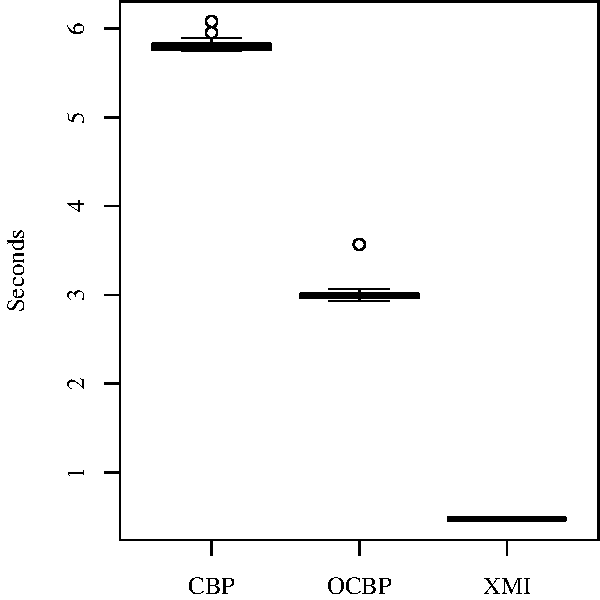
\includegraphics[width=\linewidth]{images/ol_load_time_bpmn2}
    \caption{BPMN2}
    \label{fig:load_time_bpmn2}
  \end{subfigure}
  \hfill
  \begin{subfigure}{0.325\textwidth}
    \centering
    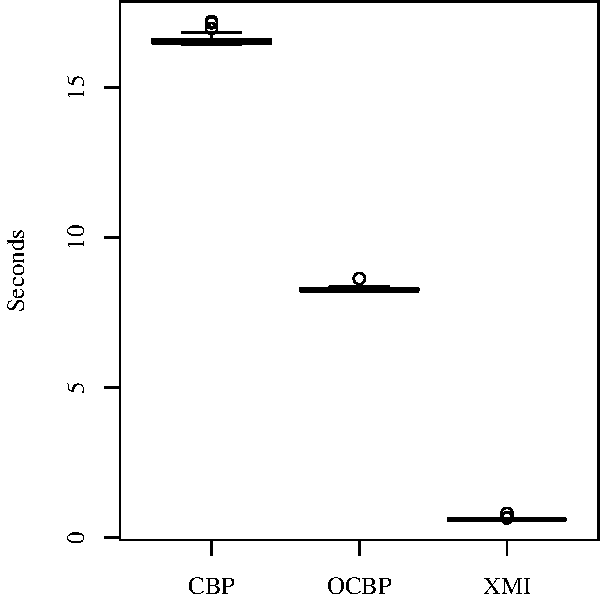
\includegraphics[width=\linewidth]{images/ol_load_time_epsilon}
    \caption{Epsilon}
    \label{fig:load_time_epsilon}
  \end{subfigure}
  \hfill
  \begin{subfigure}{0.325\textwidth}
    \centering
    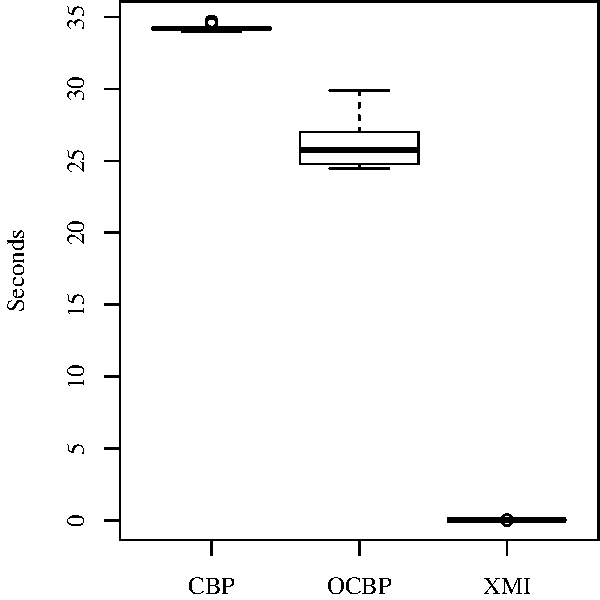
\includegraphics[width=\linewidth]{images/ol_load_time_wikipedia}
    \caption{Wikipedia}
    \label{fig:load_time_wikipedia}
  \end{subfigure}
  \caption{Results for loading a model in original CBP (CBP), optimised CBP (OCBP), and for loading a state-based (XMI) representation.}
  \label{fig:loadtime}
\end{figure}

These loading times show a considerable time saving for optimised CBP: BPMN2 was 48.02\% faster, Epsilon 50.12\% faster, and the Wikipedia page 23.63\% faster than in the original CBP implementation (all optimised CBP's $means$ are  smaller than all original CBP's $means$), which has a positive correlation to the number of ignored events. All the t-test results also show that loading times for all the persistence types are significantly different (all the $p$-$values$ $<$ 0.05). 

For reference, this work also compared CBP loading with the execution time for loading the equivalent state-based model in XMI. Figure \ref{fig:loadtime} shows that, even with the improvements delivered by the new algorithm, loading change-based models is still significantly slower than loading a state-based model (all XMI's means are smaller than other persistence types' means).

\subsection{Model Saving Time}
\label{subsec:saving_time_test}
This subsection presents the results of the saving time measurement of change-based models for each pair of the persistence types and cases, and the t-test results of their comparisons (Table \ref{table:ttest_results_savetime} and Figure \ref{fig:savetime}). As discussed in \cite{DBLP:conf/models/YohannisKP17}, CBP loading time penalties are balanced against the benefits that CBP brings, in terms of  persisting changes (saving time).

\begin{table}[ht]
\footnotesize
\centering
\caption{The t-test results of saving time comparison between original CBP (CBP), optimised CBP (OCBP), and XMI.}
\label{table:ttest_results_savetime}
\begin{tabular}
{|p{0.08\textwidth}p{0.08\textwidth}p{0.09\textwidth}|p{0.18\textwidth}p{0.10\textwidth}p{0.06\textwidth}p{0.08\textwidth}|}
\hline 

% BPMN2 Save Time
Group & Mean & SD & Comparison & t  & df & p-value \\
\hline 
\multicolumn{3}{|c|}{\textbf{BPMN2 Save Time ($s$)}} & \multicolumn{4}{c|}{\textbf{BPMN2 Save Time}}\\
CBP & 0.00097    & 123e-5 & CBP vs. XMI &  -175.58    & 22.01 & $<$ 0.05 \\  
OCBP & 0.00081   & 12e-5 & CBP vs. OCBP & 0.62 & 21.38  & 0.54 \\  
XMI & 0.30122   & 793e-5 & OCBP vs. XMI & -177.76    & 21.01  & $<$ 0.05 \\ 
\hline 

% EPSILON Save Time
\multicolumn{3}{|c|}{\textbf{Epsilon Save Time ($s$)}} & \multicolumn{4}{c|}{\textbf{Epsilon Save Time}}\\
CBP & 0.00069    & 3.4e-5 &  CBP vs. XMI & -6.01   &21.00 & $<$ 0.05 \\
OCBP & 0.00080   & 8.0e-5 & CBP vs. OCBP & 160.06 & 28.24 & $<$ 0.05 \\  
XMI & 0.40025   & 595e-5 & OCBP vs. XMI & -314.80  & 21.01  & $<$ 0.05 \\ 
\hline 

% WIKIPEDIA Save Time
\multicolumn{3}{|c|}{\textbf{Wiki Save Time ($s$)}} & \multicolumn{4}{c|}{\textbf{Wikipedia Save Time}}\\
CBP & 0.00071     & 4.9e-5 & CBP vs. XMI &  -46.19   & 21.08 & $<$ 0.05 \\ 
OCBP &0.00075   &  4.1e-5 & CBP vs. OCBP &   -3.48 & 40.77 & $<$ 0.05 \\ 
XMI &  0.01195   & 114e-5 & OCBP vs. XMI &  -46.01  & 21.06 & $<$ 0.05 \\ 
\hline
\end{tabular}
\justify
$Mean$ = average, $SD$ = standard deviation, $t$ = t-test's $t$-$value$, $df$ = degree of freedom, $p$-$value$ = significance, $s$ = the unit is seconds
\end{table}



As shown in Table \ref{table:ttest_results_savetime} and Figure \ref{fig:savetime}, the performance of the two CBP implementations is not very different. Since the significance level is 5\%, only the BPMN2 case that fails. However, the difference between the $means$ of its original CBP (0.97 ms) and optimised CBP (0.81 ms) is small. This indicates that the cost of the extra work in the optimised CBP algorithm is negligible. On the other hand, both CBP implementations are significantly faster at saving changes than state-based XMI (the $means$ of both CBP implementations are smaller than XMI's $means$, and both CBP implementations have $p$-$values$ $<$ 0.05 when compared to XMI). This is expected, as the CBP implementations only need to append the last changes to the existing model file (their performance is thus relative to the number of changes since the last save), while the XMI implementation needs to reconstruct an XML document for the entire state of the model, and replaces the contents of the model file every time (and hence its performance is relative to the size of the entire model). 

\begin{figure}[ht]
\begin{subfigure}{0.325\textwidth}
\centering
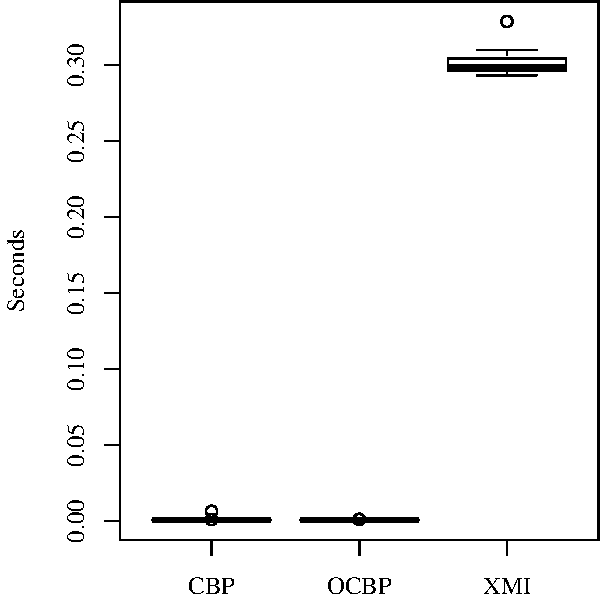
\includegraphics[width=\linewidth]{images/ol_save_time_bpmn2}
\caption{BPMN2}
\label{fig:save_time_bpmn2}
\end{subfigure}
\hfill
\begin{subfigure}{0.325\textwidth}
\centering
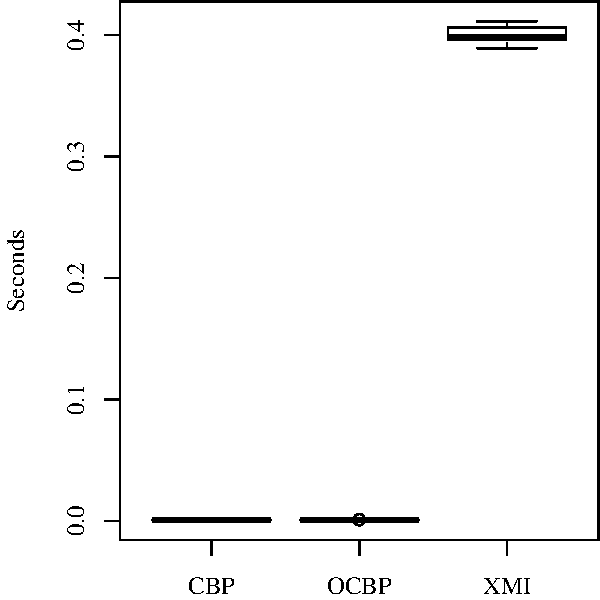
\includegraphics[width=\linewidth]{images/ol_save_time_epsilon}
\caption{Epsilon}
\label{fig:save_time_epsilon}
\end{subfigure}
\hfill
\begin{subfigure}{0.325\textwidth}
\centering
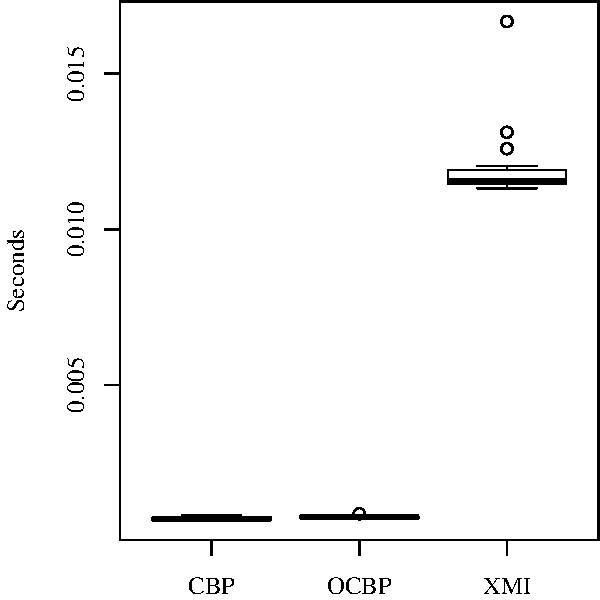
\includegraphics[width=\linewidth]{images/ol_save_time_wikipedia}
\caption{Wikipedia}
\label{fig:save_time_wikipedia}
\end{subfigure}
\caption{A comparison on time required for persisting an event between original CBP (CBP), optimised CBP (OCBP), and XMI.}
\label{fig:savetime}
\end{figure}


%\vspace{-10pt}
\subsection{Memory Footprint}
\label{subsec:memory_consumption}

\begin{table}[t]
\footnotesize
\centering
\caption{The t-test results of memory footprint comparison after loading a model between original CBP (CBP), optimised CBP (OCBP), and XMI.}
\label{table:ttest_results_load_memory}
\begin{tabular}
{|p{0.08\textwidth}p{0.08\textwidth}p{0.09\textwidth}|p{0.18\textwidth}p{0.10\textwidth}p{0.06\textwidth}p{0.08\textwidth}|}
\hline 

% BPMN2 Load Memory
Group & Mean & SD & Comparison & t  & df & p-value \\
\hline 
\multicolumn{3}{|c|}{\textbf{BPMN2 Load Memory ($M$)}} & \multicolumn{4}{c|}{\textbf{BPMN2 Load Memory}} \\
CBP & 9.76     & 76.0e-4 & CBP vs. XMI &  4,392.5   & 21.22 & $<$ 0.05 \\  
OCBP & 22.36   & 0.015 & CBP vs. OCBP & -3,695.7 & 32.28  & $<$ 0.05 \\  
XMI &  2.63   & 5.5e-4 & OCBP vs. XMI &  6,572.4    & 21.06  & $<$ 0.05 \\ 
\hline 

% EPSILON Load Memory
\multicolumn{3}{|c|}{\textbf{Epsilon Load Memory ($M$)}} & \multicolumn{4}{c|}{\textbf{Epsilon Load Memory}} \\
CBP &15.74    & 1.248 &  CBP vs. XMI & 28.16   &  41.99 & $<$ 0.05 \\
OCBP & 43.15   & 0.056 & CBP vs. OCBP & -102.9 &21.08 & $<$ 0.05 \\  
XMI & 5.05   & 1.271 & OCBP vs. XMI & 140.49  & 21.08  & $<$ 0.05 \\ 
\hline 

% WIKIPEDIA Load Memory
\multicolumn{3}{|c|}{\textbf{Wiki Load Memory ($M$)}} & \multicolumn{4}{c|}{\textbf{Wikipedia Load Memory}} \\
CBP & 2.29  & 2.4e-4 & CBP vs. XMI &   4,523.5   & 25.16 & $<$ 0.05 \\ 
OCBP & 126.48 & 0.29 & CBP vs. OCBP &   -2,009.3 & 21.00 & $<$ 0.05 \\ 
XMI &  1.52  & 7.6e-4 & OCBP vs. XMI &  2,021.8  & 21.00 & $<$ 0.05 \\ 
\hline
\end{tabular}
\justify
$Mean$ = average, $SD$ = standard deviation, $t$ = t-test's $t$-$value$, $df$ = degree of freedom, $p$-$value$ = significance, $M$ = the unit is megabytes
\end{table}

\begin{figure}[ht]
  \begin{subfigure}{0.325\textwidth}
    \centering
    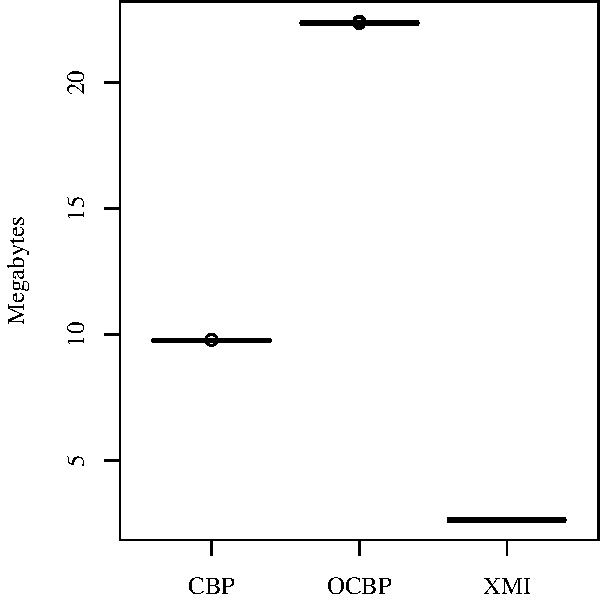
\includegraphics[width=\linewidth]{images/ol_load_memory_bpmn2}
    \caption{BPMN2}
    \label{fig:load_memory_bpmn2}
  \end{subfigure}
  \hfill
  \begin{subfigure}{0.325\textwidth}
    \centering
    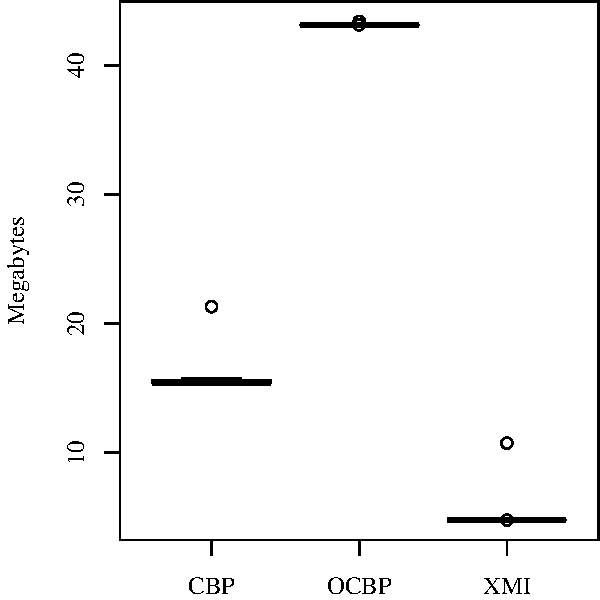
\includegraphics[width=\linewidth]{images/ol_load_memory_epsilon}
    \caption{Epsilon}
    \label{fig:load_memory_epsilon}
  \end{subfigure}
  \hfill
  \begin{subfigure}{0.325\textwidth}
    \centering
    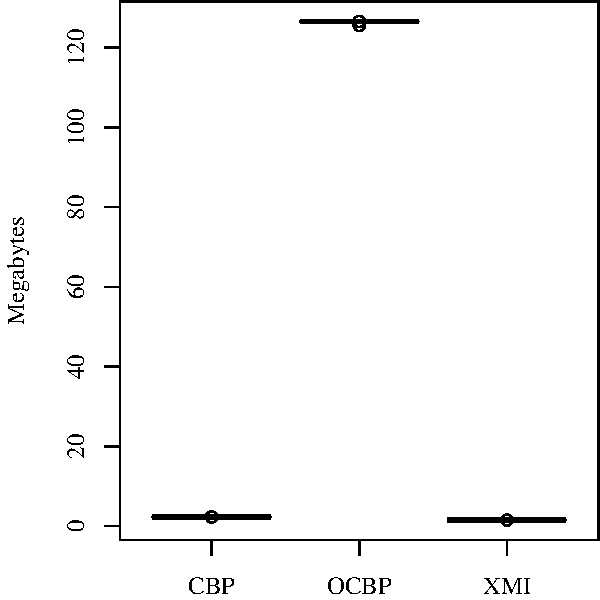
\includegraphics[width=\linewidth]{images/ol_load_memory_wikipedia}
    \caption{Wikipedia}
    \label{fig:load_memory_wikipedia}
  \end{subfigure}
  \caption{A comparison on memory footprint after loading a model between original CBP (CBP), optimised CBP (OCBP), and XMI.}
  \label{fig:loadmemory}
\end{figure}

%------------------------------

\begin{table}[ht]
\footnotesize
\centering
\caption{The t-test results of memory footprint comparison after saving an event between original CBP (CBP), optimised CBP (OCBP), and XMI.}
\label{table:ttest_results_save_memory}
\begin{tabular}
{|p{0.08\textwidth}p{0.08\textwidth}p{0.09\textwidth}|p{0.18\textwidth}p{0.10\textwidth}p{0.06\textwidth}p{0.08\textwidth}|}
\hline 

% BPMN2 Save Memory
Group & Mean & SD & Comparison & t  & df & p-value \\
\hline 
\multicolumn{3}{|c|}{\textbf{BPMN2 Save Memory ($M$)}} & \multicolumn{4}{c|}{\textbf{BPMN2 Save Memory}} \\
CBP &0.0023    & 6.3e-5 & CBP vs. XMI &  -489,170    & 41.49 & $<$ 0.05 \\  
OCBP &0.0029    & 80e-5 & CBP vs. OCBP & -3.22 & 21.26 & $<$ 0.05 \\
XMI & 8.84   & 5.6e-5 & OCBP vs. XMI & -51,180    &  21.21  & $<$ 0.05 \\ 
\hline 

% EPSILON Save Memory
\multicolumn{3}{|c|}{\textbf{Epsilon Save Memory ($M$)}} & \multicolumn{4}{c|}{\textbf{Epsilon Save Memory}}\\
CBP & 0.0025    & 18.8e-6 &  CBP vs. XMI & -4.3e\texttt{+}6   & 21.00 & $<$ 0.05 \\
OCBP & 0.0031    & 279.9e-6 & CBP vs. OCBP & -10.131 & 21.19 & $<$ 0.05 \\ %1.41e-09 \\  
XMI & 17.61   & 2.4e-6 & OCBP vs. XMI & -295,090  &21.00  & $<$ 0.05 \\ 
\hline 

% WIKIPEDIA Save Memory
\multicolumn{3}{|c|}{\textbf{Wiki Save Memory ($M$)}} & \multicolumn{4}{c|}{\textbf{Wikipedia Save Memory}} \\
CBP & 0.0025  &1.9e-5 & CBP vs. XMI &  -391,970   & 40.52 & $<$ 0.05 \\ 
OCBP &  0.0028   & 84.1e-5 & CBP vs. OCBP &  -1.75 & 21.02 &  0.094 \\ 
XMI &  2.0194   & 1.5e-5 & OCBP vs. XMI &  -11,245  & 21.01 & $<$ 0.05 \\ 
\hline
\end{tabular}
\justify
$Mean$ = average, $SD$ = standard deviation, $t$ = t-test's $t$-$value$, $df$ = degree of freedom, $p$-$value$ = significance, $M$ = the unit is megabytes
\end{table}

\begin{figure}[ht]
  \begin{subfigure}{0.325\textwidth}
    \centering
    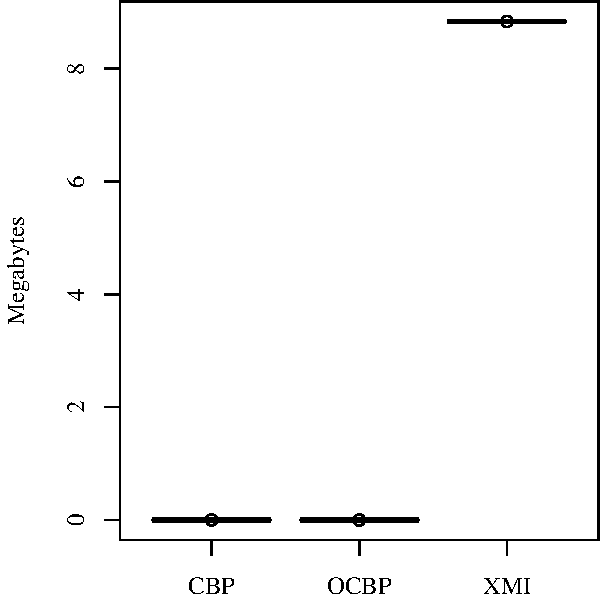
\includegraphics[width=\linewidth]{images/ol_save_memory_bpmn2}
    \caption{BPMN2}
    \label{fig:save_memory_bpmn2}
  \end{subfigure}
  \hfill
  \begin{subfigure}{0.325\textwidth}
    \centering
    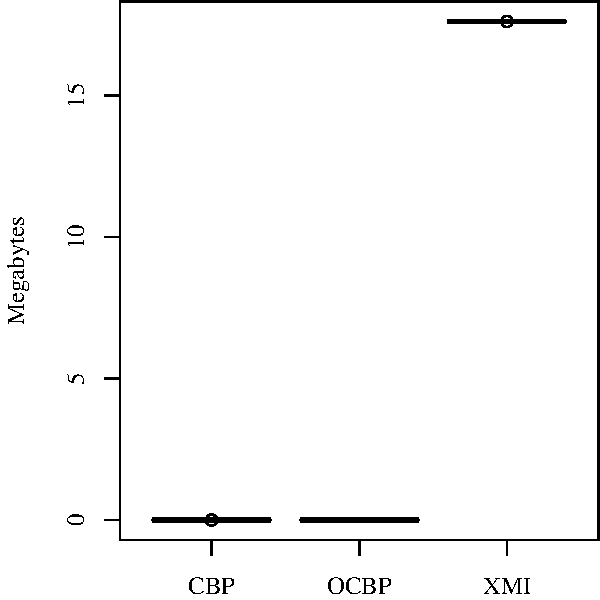
\includegraphics[width=\linewidth]{images/ol_save_memory_epsilon}
    \caption{Epsilon}
    \label{fig:save_memory_epsilon}
  \end{subfigure}
  \hfill
  \begin{subfigure}{0.325\textwidth}
    \centering
    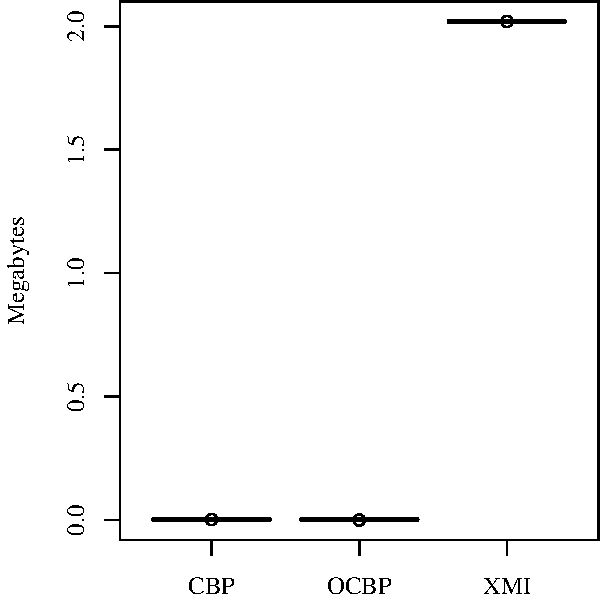
\includegraphics[width=\linewidth]{images/ol_save_memory_wikipedia}
    \caption{Wikipedia}
    \label{fig:save_memory_wikipedia}
  \end{subfigure}
  \caption{A comparison on memory footprint after persisting an event between CBP, optimised CBP, and XMI.}
  \label{fig:savememory}
\end{figure}

Using the models from the three cases, the memory footprint after loading models is presented in Table \ref{table:ttest_results_load_memory} and Figure \ref{fig:loadmemory}, and the memory footprint after persisting single changes is displayed in Table \ref{table:ttest_results_save_memory} and Figure \ref{fig:savememory}. The results show the significant memory overhead of the extra data structure when loading models (all the $means$ of optimised CBP are greater than all the $means$ of original CBP and all comparisons between both CBPs show $p$-$values$ $<$ 0.05, Table \ref{table:ttest_results_load_memory}). Both CBPs are also outperformed by XMI in terms of memory footprint when loading models (all the $means$ of XMI are smaller than all the $means$ of both CBPs and all comparisons against XMIs show all $p$-$values$ $<$ 0.05, Table \ref{table:ttest_results_load_memory}). In loading, XMI uses significantly less memory than the optimised CBP representation and performs slightly better than the original CBP.   

In terms of saving, both CBP implementations persist a single change faster than XMI indicated by their $means$ that are smaller than the $means$ of XMI, and all the CBPs' t-tests with XMI show that their differences are significant at $p$-$value$ $<$ 0.05 (Table \ref{table:ttest_results_save_memory}). The optimised CBP has a larger memory footprint than the original CBP since the means of the optimised CBP for all cases are greater than the means of the original CBP. However, their memory footprints are not very different. Even though the BPMN2 and Epsilon cases have $p$-$values$ $<$ 0.05, the differences of the $means$ of their original and optimised CBPs are small, and the Wikipedia case also shows $p$-$value$ $>$ 0.05 on its original CBP vs. optimised CBP comparison.   

\subsection{Discussion}
\label{sec:discussion}
For the original CBP loading, the total time required to load a model is $T_{CBP}$ = $T_E$ + $T_O$, where $T_E$ is the total time required to complete executing all events, and $T_O$ is the total time needed to complete other required routines (e.g. initialisation, reading files). For the optimised CBP loading, the total time to load a change-based model is reduced by the total time saved-up by ignoring superseded events $T_I$, that is $T_{OCBP}$ = $T_E$ + $T_O$ $-$ $T_I$. Thus, it is expected that optimised CBP can load a model faster than original CBP. This statement is in accordance with our finding in Section \ref{subsec:loading_time_test} that the total saved-up loading time corresponds to the number of ignored events. However, it still requires more investigation to determine the degree of their correlation, which will be addressed in our future work.

%\vspace{-5pt}
\section{Conclusions}
\label{sec:conclusions_4}
Change-based persistence can be slow when it comes to loading a model since its change records have to be replayed. This study has optimised the loading of change-based persistence by only replaying change events that affect the eventual state of a model. In other words, the replay ignores change events that are superseded by later change events.
 
This chapter has proposed an efficient algorithm and supporting data structures for the proposed optimisation. Performance is evaluated on synthesised models, with comparison against the unoptimised change-based implementation, and state-based XMI. Compared to the naive change-based representation, the optimised version shows considerable savings in terms of loading time with a negligible impact on saving time, but at the cost of a higher memory footprint. However, in terms of loading time and memory footprint, XMI outperforms both approaches but is much less efficient in saving changes. 

This chapter has addressed the first research question of this study partially, \textbf{How can models be persisted in a change-based format, and how does change-based persistence perform, compared to state-based persistence on loading and saving models?} (RQ1). Based on the evaluation results, we can identify that the performance of change-based persistence on loading models is poor compared state-based persistence. Even though it has been optimised by ignoring replaying change events that superseded by their subsequent change events, it is still significantly outperformed by loading models from their state-based persistence. It also suffers greatly on memory footprint because of the dedicated data structure employed to track change events. In terms of saving, change-based persistence shows more favourable results compared to state-based persistence since we only need to persist the recent changes applied to a model rather than saving the entire model. This condition is very favourable when we work with large models in a mature stage where mostly small changes occur. 

